\subsection{有限 Coxeter 群}

在本节中，我们将确定所有根系的同构类型，从而确定所有晶体群（第 2 节，第 5 号）。更一般地，我们先确定有限维实向量空间中由反射生成的所有有限群：这等价于确定所有有限 Coxeter 群（第五章第 4 节第 8 号），或者等价于确定所有有限阶的 Coxeter 矩阵，使其关联的双线性形式正且非退化（第五章第 4 节第 8 号定理 2）。

设 \(\mathrm{M} = (m_{ij})_{i,j\in \mathbb{I}}\) 是一个阶为 \(l\) 的有限 Coxeter 矩阵。置

\[
q _ {i j} = - \cos (\pi / m _ {i j}).
\]

回忆 \(q_{ii} = 1\)，且 \(q_{ij} = q_{ji}\) 为 0 或 \(\leqslant -1/2\)（当 \(i \neq j\) 时）。置 \(E = R^l\)，令 \((c_i)_{i \in I}\) 为 \(E\) 的典范基。记 \((x|y)\) 为 \(E\) 上与 \(M\) 关联的双线性形式（第五章第 4 节第 1 号），并记 \(q\) 为二次型 \(x \mapsto (x|x)\)（定义在 \(E\) 上）。对于 \(x = \sum_{i \in I} \xi_i x_i\)，

\[
\| x \| ^ {2} = q (x) = \sum_ {i, j \in I} q _ {i j} \xi_ {i} \xi_ {j}.
\]

记 (X, f) 为 M 的 Coxeter 图（第四章第 1 节第 9 号）。若 \(a\) 是 X 的一条边，则称 \(f(a)\) 为 \(a\) 的阶。

在本号余下部分，假设由 M 定义的 Coxeter 群 \(W(M)\)（第五章第 4 节第 3 号）是有限的，因而 q 是正且非退化的，X 是森林（第五章第 4 节第 8 号命题 8）。还假设 X 是连通的（换言之，Coxeter 群 \(W(M)\) 是不可约的），故 X 是树。

由 q 正且非退化这一条件，我们将得到关于 \(m_{ij}\) 的条件，从而能够列出相应 Coxeter 图的所有可能性；剩下的只是证明这些可能性确实能够实现，换言之，证明相应的群 W(M) 是有限的。

引理 1. 对所有 \(i\)，\(\sum_{j \neq i} q_{ij}^2 < 1\)。

令 \(J\) 为 \(j \in I\) 中满足 \(q_{ij} \neq 0\) 的元素所成的集合，换言之，满足 \(\{i, j\}\) 是 \(X\) 的一条边。若 \(j, j' \in J\) 且 \(j \neq j'\)，则 \(\{j, j'\}\) 不是一条边（否则 \(i, j, j'\) 将构成一个回路），故 \((e_j | e_{j'}) = 0\)。令 \(F = \sum_{j \in J} R e_j\)。则 \((e_j)_{j \in J}\) 是 \(F\) 的一组标准正交基。距离 \(d\)（即从 \(e_i\) 到 \(F\) 的距离）满足 \(d^2 = 1 - \sum_{j \in J} (e_i | e_j)^2 = 1 - \sum_{j \in J} q_{ij}^2 = 1 - \sum_{j \neq i} q_{ij}^2\)，故引理得证。

事实上，若 i 与 h 个其他顶点相连，则对这些顶点有 \(q_{ij}^{2} \geqslant \frac{1}{4}\)，由引理 1 得 \(\frac{h}{4} < 1\)，所以 \(h \leqslant 3\)。

引理 3. 若 \(i\) 属于 3 条边，则这些边的阶都是 3。

否则，注意到关系 \(\cos \frac{\pi}{4} = \frac{\sqrt{2}}{2}\)，便有

\[
\sum_ {j \neq i} q _ {i j} ^ {2} \geqslant \frac {1}{4} + \frac {1}{4} + (\frac {\sqrt {2}}{2}) ^ {2} = 1
\]

这不可能（引理 1）。

引理 4. 若存在一条阶 \(\geqslant 6\) 的边，则 \(l = 2\)。

事实上，设 \(\{i,j\}\) 是这样一条边。若 l \textgreater{} 2，则由于 X 连通，边 i、j 中至少有一条（设为 i）会与第三个顶点 \(j'\) 相连。注意到关系 \(\cos \frac{\pi}{6} = \frac{\sqrt{3}}{2}\)，便有

\[
\sum_ {k \neq i} q _ {i k} ^ {2} \geqslant \frac {1}{4} + (\frac {\sqrt {3}}{2}) ^ {2} = 1
\]

这不可能（引理 1）。

引理 5. 一个顶点不能属于两条不同的阶 \(\geqslant 4\) 的边。

设 \(i\) 是这样的顶点。则有 \(\sum_{j\neq i}q_{ij}^{2}\geqslant (\frac{\sqrt{2}}{2})^{2} + (\frac{\sqrt{2}}{2})^{2} = 1\)，这不可能（引理 1）。

设 \(\{i, j\}\) 是 \(X\) 的一条边。我们将定义一个新的 Coxeter 图，它将从 \(M\) 的图认同 \(i\) 和 \(j\) 后得到。其顶点集 \(I'\) 是由 \(I\) 认同 \(i\) 和 \(j\) 后得到的商集。置 \(p = \{i, j\}\)，它是 \(I'\) 的一个元素，并将 \(I\) 中异于 \(i\) 和 \(j\) 的元素与其在 \(I'\) 中的典范像认同。设 \(k, k'\) 是 \(I'\) 的两个不同元素。则在下列情形中，\(\{k, k'\}\) 是新图的一条边：

\begin{enumerate}
\def\labelenumi{\arabic{enumi})}
\item
  \(k\) 和 \(k'\) 都异于 \(p\)，且 \(\{k, k'\}\) 是 \(X\) 的一条边：在此情形，定义这条边的阶为 \(m_{kk'}\)：
\item
  \(k = p\)，且集合 \(\{i, k'\}, \{j, k'\}\) 中有一个是 \(X\) 的一条边；定义 \(\{p, k'\}\) 的阶为 \(m_{ik'}\)，若 \(\{i, k'\}\) 是 \(X\) 的一条边；并为 \(m_{jk'}\)，若 \(\{j, k'\}\) 是 \(X\) 的一条边（这两种可能性互斥，因为 \(X\) 是树）。
\end{enumerate}

令 \(M' = (m_{ij}')_{i,j \in I'}\) 为这样定义的新 Coxeter 矩阵，并置 \(q_{ij}' = -\cos \frac{\pi}{m_{ij}'}\)。则当 \(k \neq p\) 时，\(l_{pk}' = q_{ik} + q_{jk}\)。因此，若 \((\xi_i) \in \mathbf{R}^{I'}\)，

\[
\begin{array}{r l} \sum_ {k, k ^ {\prime} \in I ^ {\prime}} q _ {k k ^ {\prime}} ^ {\prime} \xi_ {k} \xi_ {k ^ {\prime}} & = \sum_ {k, k ^ {\prime} \in I} q _ {k k ^ {\prime}} \xi _ {k} \xi_ {k ^ {\prime}} + \xi_ {p} ^ {2} - \xi_ {i} ^ {2} - \xi_ {j} ^ {2} - 2 q _ {i j} \xi_ {i} \xi_ {j} \\ & = \sum_ {k, k ^ {\prime} \in I} q _ {k k ^ {\prime}} \xi _ {k} \xi_ {k ^ {\prime}} - (1 + 2 q _ {i j}) \xi_ {p} ^ {2}. \end{array} \tag {1}
\]

引理 6. 若 \(\{i,j\}\) 的阶为 3，则 \(\mathbf{W}(\mathbf{M}')\) 是有限 Coxeter 群。

事实上，\(q_{ij} = -\frac{1}{2}\)，故 (1) 变为

\[
\sum_ {k, k ^ {\prime} \in I ^ {\prime}} q _ {k, k ^ {\prime}} ^ {\prime} \xi_ {k} \xi_ {k ^ {\prime}} = \sum_ {k, k ^ {\prime} \in I} q _ {k, k ^ {\prime}} \xi_ {k} \xi_ {k ^ {\prime}}
\]

且 \((\xi_k)_{k\in I'}\mapsto \sum_{k,k'\in I'}q_{k,k'}'\xi_k\xi_{k'}\) 是正且非退化的二次型。现在只需应用第五章第 4 节第 8 号定理 2。

引理 7. 以下两种情形必有一种成立：

\begin{enumerate}
\def\labelenumi{\alph{enumi})}
\item
  X 有唯一的分叉点（第四章附录第 1 号），且 X 的所有边的阶都是 3。
\item
  X 是一条链，且至多有一条阶 \(\geqslant 4\) 的边。
\end{enumerate}

我们对 l 作归纳论证。

\begin{enumerate}
\def\labelenumi{\alph{enumi})}
\item
  假设 X 有一个分叉点 i。则 i 属于 3 条阶为 3 的边 \(\{i, k_{1}\}\)、\(\{i, k_{2}\}\)、\(\{i, k_{3}\}\)（引理 2 和 3）。若 l = 4，引理得证。否则，由于 X 连通，\(k_{1}\)（不妨设为它）属于一条不同于上述各边的边。在 M 的 Coxeter 图中认同 i 和 \(k_{1}\)。由此得到一个新图，根据引理 6 可以对它应用归纳假设。现在 i 的像 p 是新图 \(X'\) 的一个分叉点。因此 \(X'\) 没有其他分叉点，且其所有边的阶都是 3。于是 X 的所有边的阶都是 3，而 i 和 \(k_{1}\) 是其中仅有的可能分叉点。但是，若 \(k_{1}\) 是 X 的分叉点，则 p 在 \(X'\) 中至少属于 4 条边，这与引理 2 矛盾。
\item
  假设 X 没有分叉点。则 X 是一条链（第四章附录第 3 号命题 3）。设 \(\{i,j\}\) 是一条阶 \(\geqslant4\) 的边。若 l=2，引理显然成立。否则，由于 X 连通，i（不妨设为它）属于一条边 \(\{i,k\}\)，其中 \(k\neq j\)。这条边的阶为 3（引理 5）。在 M 的 Coxeter 图中认同 i 和 k。根据引理 6，可以应用归纳假设。令 p 为 i 在新图 \(X'\) 中的像。在 \(X'\) 中，\(\{p,j\}\) 是一条阶 \(\geqslant4\) 的边，所以 \(X'\) 没有其他阶 \(\geqslant4\) 的边，从而 \(\{i,j\}\) 是 X 中唯一的阶 \(\geqslant4\) 的边。
\end{enumerate}

引理 8. 设 \(i_1, i_2, \ldots, i_p\) 是 \(X\) 的顶点，使得 \(\{i_1, i_2\}, \{i_2, i_3\}, \ldots, \{i_{p-1}, i_p\}\) 是阶为 3 的边。则 \(q(\sum_{r=1}^{p} re_{t_r}) = \frac{1}{2} p(p + 1)\)。

有 \((e_{i_r}|e_{i_r}) = 1, (e_{i_r}|e_{i_{r+1}}) = -\frac{1}{2}, (e_{i_r}|e_{i_s}) = 0\)（若 \(s > r + 1\)）。因此

\[
q \left(\sum_ {r = 1} ^ {p} r e _ {i _ {r}}\right) = \sum_ {r = 1} ^ {p} r ^ {2} - 2 \sum_ {r = 1} ^ {p - 1} \frac {1}{2} r (r + 1) = p ^ {2} - \sum_ {r = 1} ^ {p - 1} r.
\]

根据《集合论》第三章第 5 节第 8 号命题 14 的推论，这等于

\[
p ^ {2} - \frac {1}{2} p (p - 1) = \frac {1}{2} p (p + 1).
\]

引理 9. 假设 X 是一条顶点为 \(1,2,\ldots,l\)、边为 \(\{1,2\},\{2,3\},\ldots,\{l-1,l\}\) 的链。

\begin{enumerate}
\def\labelenumi{(\roman{enumi})}
\tightlist
\item
  若边 \(\{2,3\},\{3,4\},\ldots,\{l-2,l-1\}\) 中有一条的阶 \(\geqslant 4\)，则该边的阶为 4，且图如下：
\end{enumerate}

\pandocbounded{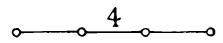
\includegraphics[keepaspectratio]{images/part002_520d8dd1.jpg}}

\begin{enumerate}
\def\labelenumi{(\roman{enumi})}
\setcounter{enumi}{1}
\tightlist
\item
  若边 \(\{1,2\}\) 的阶为 5，则图是下列图之一：
\end{enumerate}

\pandocbounded{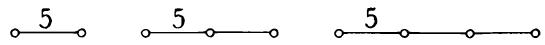
\includegraphics[keepaspectratio]{images/part002_9200390b.jpg}}

由引理 4，可设 \(l > 2\)。假设 \(\{i, i + 1\}\) 的阶为 \(\geqslant 4\)，其中 \(1 \leqslant i \leqslant l - 1\)。置

\(x = e_{1} + 2e_{2} + \dots + ie_{i}, y = e_{l} + 2e_{l - 1} + \dots + (l - i)e_{i + 1},\) 且 \(j = l - i\) .

根据引理 8，\(\| x\|^2 = \frac{1}{2} i(i + 1),\| y\|^2 = \frac{1}{2} j(j + 1)\)。另一方面，\((x|y) = ij(e_i|e_{i + 1}) = -ij\cos \frac{\pi}{m}\)，其中 \(m = 4\) 或 5（引理 4）。现在

\[
(x | y) ^ {2} <   \left\| x \right\| ^ {2} \| y \| ^ {2}.
\]

这给出

\[
\frac {1}{4} i j (i + 1) (j + 1) > i ^ {2} j ^ {2} \cos^ {2} \frac {\pi}{m}
\]

所以

\[
(i + 1) (j + 1) > 4 i j \cos^ {2} \frac {\pi}{m} \geqslant 2 i j.
\]

首先得到 \(ij - i - j - 1 < 0\)，或 \((i - 1)(j - 1) < 2\)。若

\[
1 <   i <   l - 1,
\]

则 \(1 < j < l - 1\)，所以 \(i = j = 2\)，从而 \({}^1\)

\[
9 > 16 \cos^ {2} {\frac {\pi}{m}}, \text {thus} \cos^ {2} {\frac {\pi}{m}} <   \cos^ {2} {\frac {\pi}{5}}
\]

从而 \(m = 4\)。这证明了 (i)。若 \(i = 1\) 且 \(m = 5\)，则 \(2j + 2 > 4j\frac{3 + \sqrt{5}}{8}\)，或 \(j\frac{\sqrt{5} - 1}{2} < 2\)，\(j < \sqrt{5} + 1 < 4\)，所以 \(l = j + 1 \leqslant 4\)。这证明了 (ii)。

引理 10. 若 X 有一个分叉点 i，则完全子图 \(X - \{i\}\) 是三条链的并；若 p - 1、q - 1、r - 1 是这些链的长度，则三元组 \(\{p, q, r\}\) 在置换意义下等于下列三元组之一：\(\{1, 2, 2\}\)、\(\{1, 2, 3\}\)、\(\{1, 2, 4\}\)、\(\{1, 1, m\}\)（某个 \(m \geqslant 1\)）。

顶点 \(i\) 属于 3 条边（引理 2），且没有其他分叉点（引理 7），所以完全子图 \(\mathrm{X} - \{i\}\) 是 3 条链 \(\mathrm{X}_1\)、\(\mathrm{X}_2\)、\(\mathrm{X}_3\) 的并，其中每条链都有一个与 \(i\) 在 \(\mathrm{X}\) 中相连的端点。设 \(\{i_1, i_2\}\)、\(\{i_2, i_3\}, \ldots, \{i_{p-1}, i_p\}\) 是 \(\mathrm{X}_1\) 的边，\(\{j_1, j_2\}\)、\(\{j_2, j_3\}, \ldots, \{j_{q-1}, j_q\}\) 是 \(\mathrm{X}_2\) 的边，\(\{k_1, k_2\}\)、\(\{k_2, k_3\}, \ldots, \{k_{r-1}, k_r\}\) 是 \(\mathrm{X}_3\) 的边，其中 \(i_1, j_1, k_1\) 与 \(i\) 在 \(\mathrm{X}\) 中相连。可设 \(p \geqslant q \geqslant r \geqslant 1\)。置

\[
\begin{array}{l} x = e _ {i _ {p}} + 2 e _ {i _ {p - 1}} + \dots + p e _ {i _ {1}} \\ y = e _ {j _ {q}} + 2 e _ {j _ {q - 1}} + \dots + q e _ {j _ {1}} \\ z = e _ {k _ {r}} + 2 e _ {k _ {r - 1}} + \dots + r e _ {k _ {1}}. \end{array}
\]

由于 X 的所有边的阶都是 3（引理 7），由引理 8 得 \(\| x\|^2 = \frac{1}{2} p(p + 1)\)、\(\| y\|^2 = \frac{1}{2} q(q + 1)\)、\(\| z\|^2 = \frac{1}{2} r(r + 1)\)。另一方面，\(e_i\) 与 \(e_{i_2}, e_{i_3}, \ldots, e_{i_p}\) 正交，故 \((e_i|x) = p(e_i|e_{i_1}) = -\frac{1}{2} p\)；同理 \((e_i|y) = -\frac{1}{2} q\)、\((e_i|z) = -\frac{1}{2} r\)。单位向量 \(\| x\|^ {-1}x\)、\(\| y\|^ {-1}y\)、\(\| z\|^ {-1}z\) 两两正交，且 \(e_i\) 不属于它们生成的子空间 F；从 \(e_i\) 到 F 的距离的平方为

\[
\begin{array}{r l} 1 - (e _ {i} | \frac {x}{\| x \|}) ^ {2} - (e _ {i} | \frac {y}{\| y \|}) ^ {2} - (e _ {i} | \frac {z}{\| z \|}) ^ {2} \\ & = 1 - \frac {1}{2} \frac {p}{p + 1} - \frac {1}{2} \frac {q}{q + 1} - \frac {1}{2} \frac {r}{r + 1} \\ & = 1 - \frac {1}{2} + \frac {1}{2} \frac {1}{p + 1} - \frac {1}{2} + \frac {1}{2} \frac {1}{q + 1} - \frac {1}{2} + \frac {1}{2} \frac {1}{r + 1}. \end{array}
\]

由于此量为 \(>0\)，有

\[
(p + 1) ^ {- 1} + (q + 1) ^ {- 1} + (r + 1) ^ {- 1} > 1.\tag{4}
\]

因此 \(3(r + 1)^{-1} > 1\)，所以 \(r < 2\)，最后 \(r = 1\)。于是由 (4) 得

\[
(p + 1) ^ {- 1} + (q + 1) ^ {- 1} > \frac {1}{2}\tag{5}
\]

故 \(2(q + 1)^{-1} > \frac{1}{2}\)，所以 \(q \leqslant 2\)。最后，若 \(q = 2\)，由 (5) 得

\[
(p + 1) ^ {- 1} > \frac {1}{6}. \quad \text { hence } p \leqslant 4.
\]

定理 1. 任一不可约有限 Coxeter 系统 (W.S) 的图同构于下列图之一：

\pandocbounded{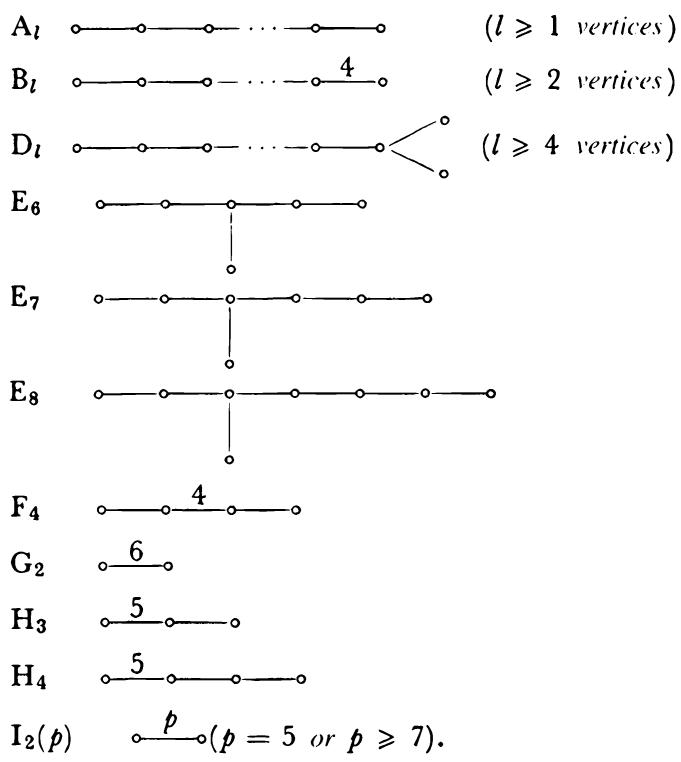
\includegraphics[keepaspectratio]{images/part002_677d99d4.jpg}}

这些图中任意两个都不同构。

事实上，设 \(\mathrm{W} = (m_{ij})\) 是 (W,S) 的 Coxeter 矩阵，且 \(l = \operatorname{Card}(S)\)。若某个 \(m_{ij}\) 为 \(\geqslant 6\)，则 l = 2（引理 4），且 (W,S) 的 Coxeter 图是 \(G_{2}\) 型或 \(I_{2}(p)\) 型，其中 \(p \geqslant 7\)。现在假设所有 \(m_{ij} \leqslant 5\)。

\begin{enumerate}
\def\labelenumi{\alph{enumi})}
\item
  若 \(m_{ij}\) 不全都等于 3，则 (W.S) 的图 X 是一条链，且恰有一个 \(m_{ij}\) 等于 4 或 5（引理 7）。若某个 \(m_{ij}\) 等于 5，则引理 9 表明我们得到 \(H_{3}\)、\(H_{4}\) 或 \(I_{2}(5)\) 型之一。若某个 \(m_{ij}\) 等于 4，则引理 9 表明我们得到 \(B_{l}\) 或 \(F_{4}\) 型之一。
\item
  现在假设所有 \(m_{ij}\) 都等于 3。若 X 是一条链，则 Coxeter 图是 \(A_{l}\) 型。否则，引理 10 表明它是 \(E_{6}\)、\(E_{7}\)、\(E_{8}\) 或 \(D_{l}\) 型。
\end{enumerate}

显然，所列 Coxeter 图中任意两个都不同构。

反之：

定理 2. 定理 1 中由 Coxeter 图 \(\mathbf{A}_l, \mathbf{B}_l, \ldots, \mathbf{I}_2(p)\) 定义的 Coxeter 群是有限的。

对于 \(I_{2}(p)\) 这显然成立，因为相应的群是阶为 2p 的二面体群（第四章第 1 节第 9 号）。对于 \(H_{4}\)，相应的二次型

为

\[
\begin{array}{r l} & \xi_ {1} ^ {2} + \xi_ {2} ^ {2} + \xi_ {3} ^ {2} + \xi_ {4} ^ {2} - \xi_ {1} \xi_ {2} - \xi_ {2} \xi_ {3} - 2 (\cos \frac {\pi}{5}) \xi_ {3} \xi_ {4} \\ & = \xi_ {1} ^ {2} + \xi_ {2} ^ {2} + \xi_ {3} ^ {2} + \xi_ {4} ^ {2} - \xi_ {1} \xi_ {2} - \xi_ {2} \xi_ {3} - \frac {1 + \sqrt {5}}{2} \xi_ {3} \xi_ {4} \\ & = (\xi_ {2} - \frac {\xi_ {1} + \xi_ {3}}{2}) ^ {2} + (\xi_ {4} - \frac {1 + \sqrt {5}}{4} \xi_ {3}) ^ {2} + \frac {3}{4} (\xi_ {1} - \frac {1}{3} \xi_ {3}) ^ {2} + \frac {7 - 3 \sqrt {5}}{24} \xi_ {3} ^ {2}. \end{array}
\]

由于 \(7 - 3\sqrt{5}\) 为 \textgreater0，此形式正且非退化，故相应的 Coxeter 群是有限的。\(H_{3}\) 所对应的情形也如此，因为它同构于前一个群的子群（第四章第 1 节第 8 号）。

对于 \(A_{l}\)、\(B_{l}, \ldots, G_{2}\) 型，我们将在第 5 至 13 号中构造以相应群为韦伊群的根系。我们将看到，这些群不仅有限，而且是晶体群（第 2 节，第 5 号）。

